\documentclass[a4paper,11pt]{report}
\usepackage[utf8]{inputenc}
\usepackage[T1]{fontenc}
\usepackage{todonotes}
\usepackage{appendix}
\usepackage{longtable}
\usepackage{amsmath}
\usepackage{amssymb}
\usepackage{tikz}
\usepackage{pgf}
\usepackage{geometry}
\usepackage{paralist}
\usepackage{hyperref}
\usepackage[format=hang]{subfig}
\usepackage{graphicx}
\usepackage{caption}
\usepackage{color}
\usepackage{float}
\usepackage{natbib}
\usepackage{apalike}
\usepackage[svgnames]{color}
\usepackage{commath}
\usepackage{listings}
\usepackage[boxed,ruled,lined,algochapter]{algorithm2e}
\usepackage[boxed,ruled,lined,algochapter]{algorithmic}


\newcommand{\Colin}[0]{\textsc{Colin }}

\pagenumbering{roman}
\geometry{a4paper,left=25mm,right=20mm, top=20mm, bottom=20mm} 

\linespread {1.25}

\let\oldsqrt\sqrt
\def\sqrt{\mathpalette\DHLhksqrt}
\def\DHLhksqrt#1#2{%
\setbox0=\hbox{$#1\oldsqrt{#2\,}$}\dimen0=\ht0
\advance\dimen0-0.2\ht0
\setbox2=\hbox{\vrule height\ht0 depth -\dimen0}%
{\box0\lower0.4pt\box2}}

\usetikzlibrary{calc}
\usepgfmodule{plot}
\usepgflibrary{plothandlers}
\usetikzlibrary{mindmap}
\usetikzlibrary{trees}
\usetikzlibrary{arrows}
\usetikzlibrary{automata}
\usetikzlibrary{positioning}
\usetikzlibrary{decorations}
\usetikzlibrary{backgrounds}
\usetikzlibrary{decorations.pathreplacing}



\bibliographystyle{apalike}


\makeatletter
\@addtoreset{lstlisting}{chapter}
\@addtoreset{table}{chapter}
\@addtoreset{figure}{chapter}
\makeatother

\begin{document}


\begin{titlepage}

\begin{center}
\ \\
\vspace{100pt}
\Huge{\textbf{Colin}}

\Large{User Manual for version 0.2.0-0
}

\vspace{100pt}
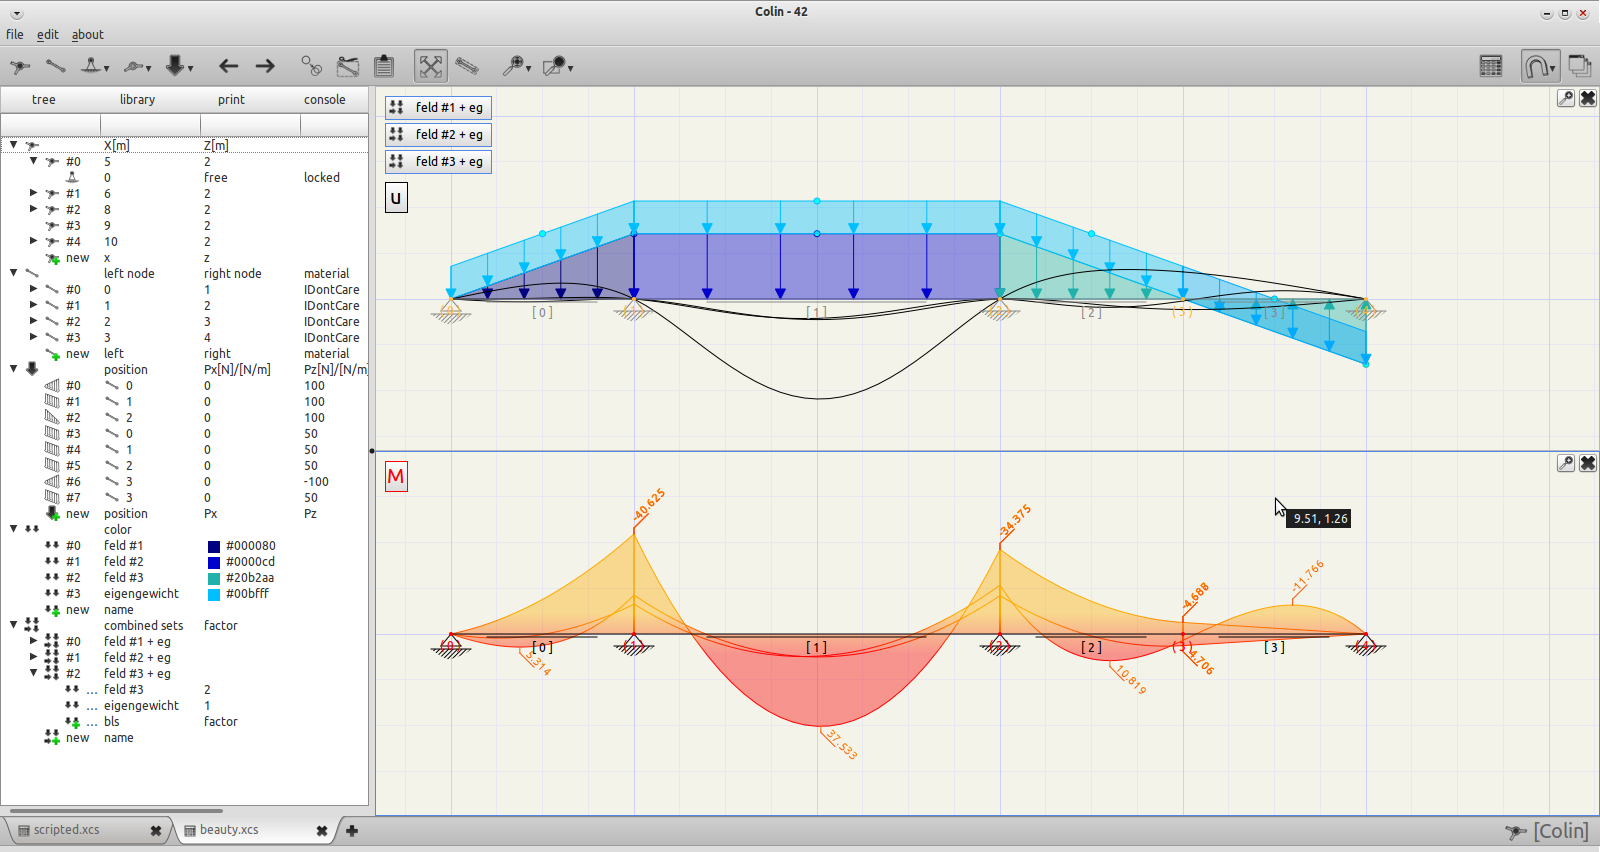
\includegraphics[width=\textwidth]{../pictures/title.png}
\end{center}
\vspace{40pt}
\begin{center}
\large{an open source structural analysis application}
\end{center}

\end{titlepage}
\clearpage


\begin{minipage}[h]{0.25\textwidth}
\begin{center}

\includegraphics[height=3cm]{./pictures/clazzes2.jpg}
\end{center}
\end{minipage}
\begin{minipage}[h]{0.75\textwidth}
\textbf{\large{Colin is a Clazzes.org Project.}}
\vspace{8pt}\\
www.clazzes.org
\end{minipage}
\vspace{20pt}
\hline
\vspace{20pt}
\begin{minipage}[h]{0.25\textwidth}
\begin{center}

\includegraphics[height=3cm]{./pictures/qt_ambassador_logo.png}
\end{center}
\end{minipage}
\begin{minipage}[h]{0.75\textwidth}
%\begin{flushright}
\textbf{\large{Colin is Part of the Qt Ambassador Programm.}}
\vspace{8pt}\\
qt.nokia.com/qtambassador
%\end{flushright}
\end{minipage}
\vspace{20pt}
\hline
\vspace{20pt}
\begin{minipage}[h]{0.25\textwidth}
\begin{center}

\includegraphics[height=3cm]{./pictures/logo2-icon_128x128.png}
\end{center}
\end{minipage}
\begin{minipage}[h]{0.75\textwidth}
%\begin{flushright}
\textbf{\large{With support and help from ITEG IT-Engineers}}
\vspace{8pt}\\
www.iteg.at
%\end{flushright}
\end{minipage}
\ \\

\vspace{250pt}


\begin{center}
	
\includegraphics[scale=0.5]{./pictures/280px-CreativeCommond_logo_trademark.png}
	
\includegraphics[scale=0.5]{./pictures/64px-Cc-by_new.png}
	
\includegraphics[scale=0.5]{./pictures/64px-Cc-sa_white.png}
\end{center}
\begin{center}This work is licensed under a Creative Commons Attribution-ShareAlike 3.0 License.\end{center}




\clearpage
\ \\
\vspace{470pt}
\ \\
Copyright \copyright 2011 Matthias Rauter(\href{mailto:matthias.rauter@student.uibk.ac.at}{matthias.rauter@student.uibk.ac.at})\\
\vspace{20pt} \ \\
\Colin is free software; you can redistribute it and/or modify it under the terms of the GNU General Public License as published by the Free Software Foundation; either version 3 of the License, or (at your option) any later version.\\
\Colin is distributed in the hope that it will be useful, but \textbf{without any warranty}; without even the implied warranty of \textbf{merchantability} or \textbf{fitness for a particular purpose}. See the GNU General Public License for more details.\\
You should have received a copy of the GNU General Public License along with this program; if not, see \url{http://www.gnu.org/licenses/}.


\clearpage

\tableofcontents


\clearpage
\pagenumbering{arabic}

\chapter{What's Colin?}
\label{cha:colin}

\Colin is an structural analysis application. It's availible under the term of the GNU General Public License\footnote{\url{http://www.gnu.org/licenses/}}. Unlike most other licenses, the GNU GPL offers you the following:
\begin{enumerate}
	\item [0] the freedom to use the software for any purpose,
	\item [1] the freedom to change the software to suit your needs,
	\item [2] the freedom to share the software with your friends and neighbors, and
	\item [3] the freedom to share the changes you make.
\end{enumerate}\\
The source code of \Colin is availible at clazzes.org. Feel free to explore our SVN\footnote{\url{http://subversion.tigris.org/}} repository at \url{http://svn.clazzes.org/svn/colin/}. Prebuild packages are available for Debian GNU/Linux and Windows. Users of other operation systems can compile it themselves.\\

\Colin is limited to two dimensional structures and an analytical, linear analysis of those. Structures can be statically indeterminate. The following elements can be used to describe the physical structure:
\begin{itemize}
	\item \textit{Nodes} and \textit{Beams} to describe the geometry and physical properties
	\item \textit{Supports}, including springs and rotated supports
	\item \textit{Hinges} of all kind, including springs
	\item \textit{Loads}, including Nodal loads, linear distributed loads, temperature loads
	\item \textit{Basic Load Sets} and \textit{Combined Load Sets}
\end{itemize}\\
Besides, \Colin offers the following additional features for an easy handling:
\begin{itemize}
	\item complete CAD environment
	\item object, grid and orthogonal snap
	\item saving to XML
	\item unlimited undo/redo
	\item copy'n`paste
	\item printing
	\item table like editing in a tree representation
	\item JavaScript Engine including a console
\end{itemize}

\section{getting started on Linux}
\label{sec:startLinux}

If you use a Debian GNU/Linux based distribution, you can use our Debian repository. Debian GNU/Linux based distributions use the *.deb format to install packages. Debian, Ubuntu and Linux Mint should work with our packages. For distribution witch use *.rpm packages see section~\ref{sec:startOther}.\\

First you need to trust our archiver key. You can do so by opening a terminal and typing:
\begin{lstlisting}[frame=single, breaklines=true, basicstyle=\small]
wget https://www.clazzes.org/gpg/pba-archiver.clazzes.org.asc -O - | sudo apt-key add - 
\end{lstlisting}
Then you can add our repository to the software sources. To do so, open the \textit{Software Center}. To edit your software sources there, open the \textit{Edit} menu in the menubar and click on \textit{Software  Sources...} there.\\
A new Window should appear. Activate the \textit{Other Software} tab there. Click \textit{Add...} there and enter the following text, depending on your operation systems version:

\begin{itemize}
	\item Ubuntu Lucid Lynx 10.04 or newer and the corresponding Linux Mint
\begin{lstlisting}[frame=single, breaklines=true, basicstyle=\small]
deb http://deb.clazzes.org/ubuntu lucid-colin-1 main  
\end{lstlisting}
	\item Debian Squeeze 6
\begin{lstlisting}[frame=single, breaklines=true, basicstyle=\small]
deb http://deb.clazzes.org/debian squeeze-colin-1 main
\end{lstlisting}
\end{itemize}

After updating \textit{apt-get} you should be able to install \Colin.



\section{getting started on Windows}
\label{sec:startWindows}

You can find Windows Setups in our download area at clazzes.org: \url{http://download.clazzes.org/colin/testing/}. *x64* marks the 64 bit version, *x86* the 32 bit version. Download the right version for your Windows. You can install it by executing the Setup. \\

\textbf{note:}
\begin{center}
\textbf{Other than on Linux, the Windows version of \Colin does not get updated automatically. Please take look at clazzes.org from time to time to watch out for newer versions of \Colin. Or simply switch to Linux ;)}
\end{center}

\section{getting started on other OS}
\label{sec:startOther}

If you are using an OS for witch no packages are provided, you can download the source from our SVN repository and compile it your self. \Colin should work on most operation systems, including all UNIX like operation systems and OS X. To get \Colin compiled take a look at chapter~\ref{cha:compile}.\\
A version for OS/2 has already been compiled by some else. You can find it at ecomstation.it\footnote{\url{http://www.ecomstation.it/ecsoft2/prog.php?progid=1795&name=Colin&sys=os2+ecomstation}}. Please note that i don't keep this build up-to-date.


\chapter{Objects}
\label{cha:objects}

This chapter gives a quick overview over the objects in \Colin.

\section{Struct}
This object defines structures. It contains all Nodes, Beams, Loads, etc. 

\section{Node}
A Node defines the geometry of structures in \Colin. It contains the coordinates \textit{x} and \textit{z}. Supports can be added to Nodes.

\section{Support}
Supports define the boundary conditions of nodes. Use these to lock the displacement of nodes.

\section{Beam}
These objects represent the beams of the structure. They are spanned between two nodes. Beams contain a reference to their left and right node, their cross section and their material. Besides, hinges can be assigned to beams to define boundary conditions.

\section{Hinge}
Hinges define boundary conditions of beams. 

\section{Loads}
These objects define the load on the structure.

\subsection{Nodal Load}
A simple load on a node.

\subsection{Moment}
A moment on a node.

\subsection{Distributed Loads}
Linear distributed or uniformly distributed loads on beams.

\subsection{Temeperatur Loads}
Loads due to temperature changes or temperature differences.
 
\subsection{Double Load} 
Loads between the left and right side of a hinge.

\section{Basic Load Set}
Loads can be assigned to Basic Load Sets (BLS) to group them.

\section{Combined Load Set}
Combine groups of loads for the calculation of many cases in once.

\section{Material}
The material defines material properties of beams, \textit{stiffness} E and \textit{thermal expansion coefficient} $\alpha_T$.

\section{Cross Section}
Cross Sections define the geometry of beams in their local y-z plane,  \textit{height} h, \textit{area} A and \textit{second moment of area} I.

\chapter{Graphical User Interface}

This chapter gives an overview over the Graphical User Interface (GUI) of Colin.

\section{Workspace}
\label{sec:workspace}

Here a quick overview over the Workspace. This is the part of the GUI you are actually working with. The different parts are explained in depth later.
\begin{figure}[H]
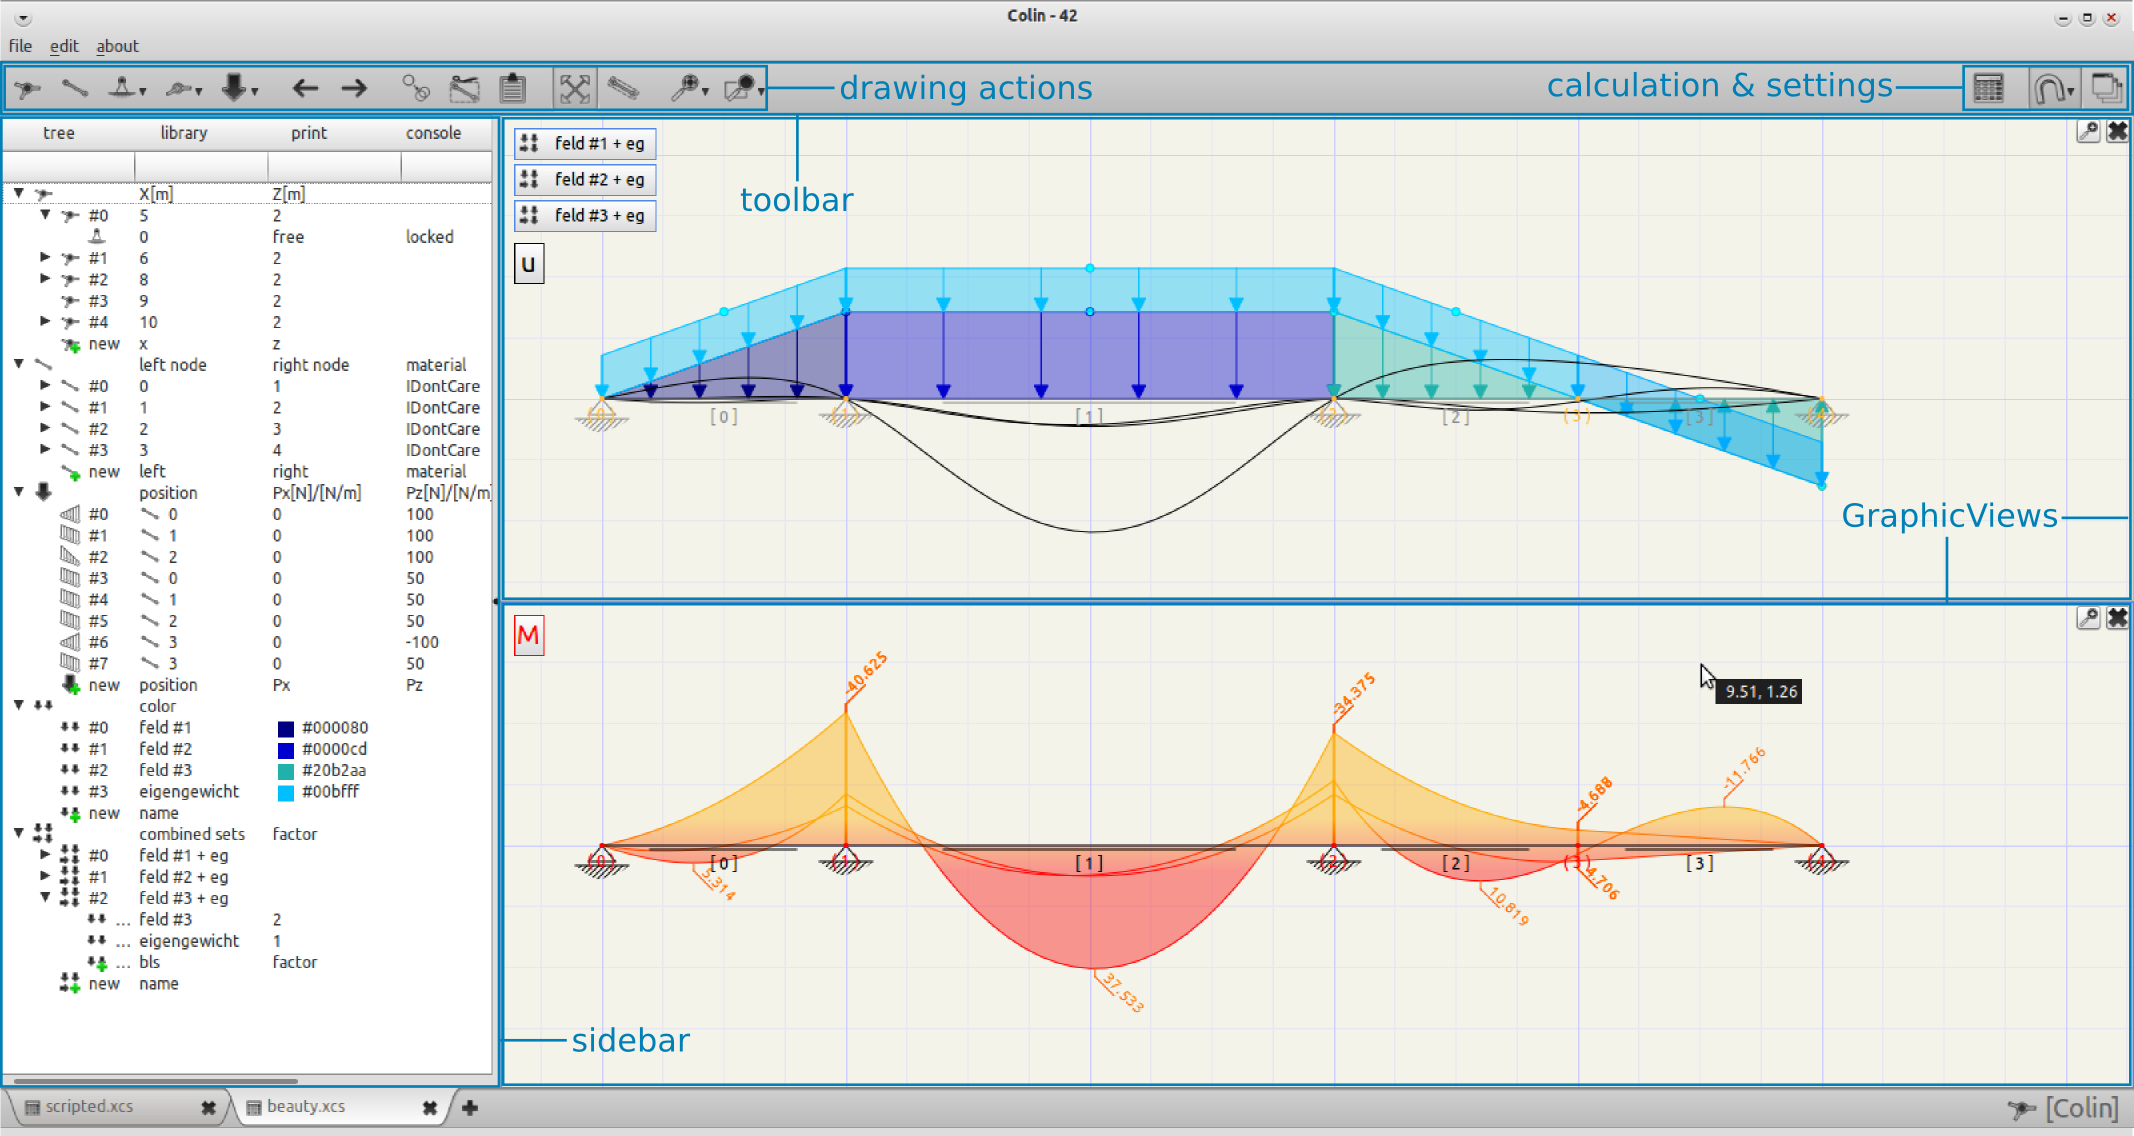
\includegraphics[width=\textwidth]{./pictures/workspace_overlay.png}
\caption{Workspace}
\label{pic:workspace}
\end{figure}

Figure~\ref{pic:workspace} shows the elements of the workspace:
\begin{itemize}
	\item Menubar: On the top of the Mainwindow. See section~\ref{sec:menubar}.
	\item Toolbar: 
	\begin{itemize}
		\item drawing actions: these actions interact with the GraphicsView
		\item calculation and settings: here you can find some quick settings for the snap and the shown windows. also the action to calculate forces of the structure is placed here.
	\end{itemize}
	See section~\ref{sec:toolbar}.
	\item Sidebar: the sidebar contains additional views and widgets:
	\begin{itemize}
		\item tree: shows a tree which represents the current structure. See section~\ref{ssec:tree}.
		\item library: gives access to the library (stored materials and cross sections). See section~\ref{ssec:library}.
		\item print: shows a printing dialog. See section~\ref{ssec:printingwidget}.
		\item console: a console which interprets Javascript and  See section~\ref{ssec:console}.
	\end{itemize}
	See section~\ref{sec:sidebar}.
	\item GraphicsView: Here you can see the graphical representation of a structure and the results of the calculation. Also, you can draw new elements and manipulate existing ones. See section~\ref{sec:graphical}.
	\item Tabbar: Shows the opened files. See section~\ref{sec:tabbar}.
\end{itemize}

\section{Menubar}
\label{sec:menubar}
The menubar is placed on top of the Mainwindow on most operation systems. The \textit{file} menu contains some basic actions to organize, such as \textit{open} and \textit{save} (see figure~\ref{pic:filemenu}). The \texitit{edit} menu contains some additional actions to manipulate the current file (see figure~\ref{pic:editmenu}) which are not present in the toolbar (see section~\ref{sec:toolbar}. You can activate these action by pressing the shortcut. It's visible next to the corresponding action.

\begin{minipage}[b]{\textwidth/2}
\begin{figure}[H]
\begin{center}
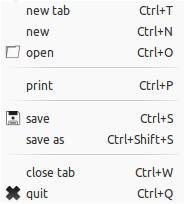
\includegraphics[scale=0.6]{./pictures/filemenu.png}
\caption{menu: \textit{file}}
\label{pic:filemenu}
\end{center}
\end{figure}
\end{minipage}
\begin{minipage}[b]{\textwidth/2}
\begin{figure}[H]
\begin{center}
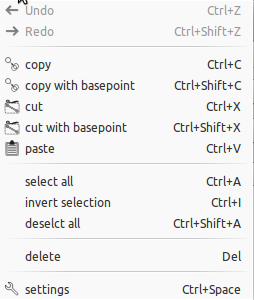
\includegraphics[scale=0.6]{./pictures/editmenu.png}
\caption{menu: \textit{edit}}
\label{pic:editmenu}
\end{center}
\end{figure}
\end{minipage}


\subsection{file menu}
Here a quick overview over the action present in this menu:
\begin{itemize}
	\item \textit{new tab}: shows the start page
	\item \textit{new}: creates a new empty file
	\item \textit{open}: open a file on your computer
	\item \textit{print}: launches the print dialog
	\item \textit{save}: saves the current file. Overwrites any other version. If the file was not saved before, a dialog appears where you can enter the designated filename
	\item \texit{save as}: saves the current file. Asks for a filename.
	\item \textit{close tab}: closes the current tab. Asks for saving the file has been edited.
	\item \textit{quit}: closes the application. Asks for saving before.
\end{itemize}

\subsection{edit menu}
A quick overview over the \textit{edit} menu. 
\begin{itemize}
	\item \textit{Undo}: undo the last change.
	\item \textit{Redo}: redo the last undone change.
	\item \textit{copy}: copy all currently selected objects to the clipboard. 
	\item \textit{copy with basepoint}: like copy, but when pasting form clipboard, you can chose the position where it gets inserted in relation to the given basepoint. More in section~\ref{sec:graphical}.
	\item \textit{cut}: like copy, deletes original objects.
	\item \textit{cut with basepoint}: like copy with basepoint, deletes original objects.
	\item \textit{paste}: paste from clipboard.
	\item \textit{select all}: selects all elements of the current structures.
	\item \textit{invert selection}: selects all elements of the current structure which are not selected and vise versa.
	\item \textit{deselect all}: removes selection state from all objects.
	\item \textit{delete}: deletes the currently selected objects.
	\item \textit{settings}: launces the settings page.
\end{itemize}
\section{Tabbar}
\label{sec:tabbar}
This bar can be found on the buttom of the Colin GUI. You can see all open files and active them by clicking on them. Press the cross to close a tab. Press "+" to open a new tab.
\begin{figure}[H]

\includegraphics[width=\textwidth]{./pictures/tabbar.png}
\caption{tabbar}
\label{pic:tabbar}
\end{figure}

\section{Toolbar}
\label{sec:toolbar}

The toolbar contains the most used actions. Icons with a triangle besides them are expandable. You can trigger a menu with more options by keeping the button pressed long. When moving the mouse over a icon a tooltip with some basic informations of the usage appears. 

\begin{figure}[H]

\includegraphics[width=\textwidth]{./pictures/toolbar.png}
\caption{toolbar}
\label{pic:toolbar}
\end{figure}

Here the actions in the toolbar from left to right.
\subsection{Nodes}
When activated, you can draw Nodes by clicking on the designated position in the GraphicsView. When you click on a beam, the beam gets spitted at the clicked position, when clicking on 2 crossing beams, the get both splitted and connected with a new node.

\subsection{Beams}
When activated, you can draw Beams, by clicking on the designated nodes in the GraphicView. If you do not click on a node, a new node will be created. Material and cross section are chosen automatically. You can set the material and cross section of beams created like this in the library widget (see section~\ref{ssec:library}). You can edit them afterwards too. This is shown in section~\ref{sec:graphical} (by using the GraphicView) and in section~\ref{ssec:tree} (by using the tree representation).

\subsection{Supports}
\begin{minipage}[h]{4cm}
\begin{figure}[H]
\begin{center}
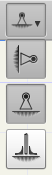
\includegraphics[scale=0.6]{./pictures/support_opt.png}
\caption{options}
\label{pic:support_opt}
\end{center}
\end{figure}
\end{minipage}
\begin{minipage}[h]{\textwidth-4cm}
When activated, you can add supports to nodes by clicking on the in the GraphicsView. Keep the mouse button pressed to get access to more settings. The buttons as shown in figure~\ref{pic:support_opt} appear. Here you can set the basic form of the support which gets added to a nodes by clicking on them:
\begin{trivlist}
	\item[] 
\includegraphics[scale = 0.5]{../../icons/bearingH.png} horizontal support: the horizontal displacement will be zero
	\item[] 
\includegraphics[scale = 0.5]{../../icons/bearing.png} vertical support: the vertical displacement of the node will be zero
	\item[] 
\includegraphics[scale = 0.5]{../../icons/bearingM.png} rotational support: the rotation of the node will be zero
\end{trivlist}
You can choose any combination of these 3 basic supports. To use springs as supports and for rotated supports see section~\ref{ssec:tree}.
\end{minipage}

\subsection{Hinges}

\begin{minipage}[h]{4cm}
\begin{figure}[H]
\begin{center}

\includegraphics[scale=0.6]{./pictures/hinge_opt.png}
\caption{options}
\label{pic:hinge_opt}
\end{center}
\end{figure}
\end{minipage}
\begin{minipage}[h]{\textwidth-4cm}
When activated, you can add hinges to beams. Click on a beam to add a hinge at the designated position of the beam. Click near the left or right node of a beam to put the hinge to the right or left end of the beam. Keep the button pressed to get access to more settings. You can choose the the type of hinge by clicking on the respective button:
\begin{trivlist}
	\item[] 
\includegraphics[scale = 0.5]{../../icons/jointN.png} normal force on the respective position will be zero.
	\item[] 
\includegraphics[scale = 0.5]{../../icons/jointQ.png} shear force on the respective position will be zero.
	\item[] 
\includegraphics[scale = 0.5]{../../icons/joint.png} moment on the respective position will be zero.
\end{trivlist}
If you want a sprint between the left and right side of a hinge take a look in section~\ref{ssec:tree}.
\end{minipage}

\subsection{Loads}

\begin{minipage}[h]{4cm}
\begin{figure}[H]
\begin{center}

\includegraphics[scale=0.6]{./pictures/load_opt.png}
\caption{options}
\label{pic:load_opt}
\end{center}
\end{figure}
\end{minipage}
\begin{minipage}[h]{\textwidth-4cm}
When activated you can add loads to the structure. Most of the actions here need two clicks to create a load. Figure~\ref{pic:drawload} shows the two required clicks for an uniformly distributed load. Keep the button pressed to get access to more settings. The possible types of loads:
\begin{trivlist}
	\item[] 
\includegraphics[scale = 0.5]{../../icons/load.png} nodal lode. Click on a node in the GraphicsView to specify the position of the load. The second click sets the values $P_x$ and $P_z$ of the load and completes the input.
	\item[] 
\includegraphics[scale = 0.5]{../../icons/moment.png} moment. Click on a node in the GraphicsView to specify the position of the moment. The second click sets the value $M$ of the load and completes the input.
	\item[] 
\includegraphics[scale = 0.5]{../../icons/ustload.png} uniformly distributed load. Click on a beam to specify the position of the load. The second click sets the values $P_x$ and $P_z$ of the load and completes the input.
	\item[] 
\includegraphics[scale = 0.5]{../../icons/istload.png} increasing linear load. just like the uniformly distributed load.
	\item[] 
\includegraphics[scale = 0.5]{../../icons/dstload.png} decreasing linear load. just like the uniformly distributed load.
	\item[] 
\includegraphics[scale = 0.5]{../../icons/temp.png} temperature load. Click on a beam to specify the designated position of the temperature load. The widget as shown in figure~\ref{pic:tempwidget} in form of a thermometer appears. You can switch between temperature change and temperature difference (between top and bottom of the cross section) by clicking the button besides the thermometer or pressing the left and right keys ($\leftarrow$ and $\rightarrow$) on your keyboard. You can set the temperature difference by clicking on the thermometer (the scale is adapted automatically) or with the up and down keys ($\uparrow$ and $\downarrow$) of your keyboard. \textbf{Complete the input with the \textit{Enter} key.}
	\item[] 
\includegraphics[scale = 0.5]{../../icons/doubleL.png} double loads between the left and right side of a hinge.
\end{trivlist}
\end{minipage}

\begin{minipage}[b]{\textwidth/2}
\begin{figure}[H]
\begin{center}
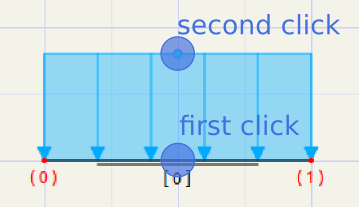
\includegraphics[height=3cm]{./pictures/drawload_overlay.png}
\caption{the two required clicks to draw a load}
\label{pic:drawload}
\end{center}
\end{figure}
\end{minipage}
\begin{minipage}[b]{\textwidth/2}
\begin{figure}[H]
\begin{center}
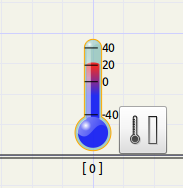
\includegraphics[height=3cm]{./pictures/temp_wid.png}
\caption{adding a temperature load}
\label{pic:tempwidget}
\end{center}
\end{figure}
\end{minipage}

\subsection{Undo/Redo}
\begin{minipage}[h]{4cm}
\begin{figure}[H]
\begin{center}

\includegraphics[scale=0.6]{./pictures/undoredotoolbar.png}
\caption{Undo}
\label{pic:undoredotoolbar}
\end{center}
\end{figure}
\end{minipage}
\begin{minipage}[h]{\textwidth-4cm}
\begin{trivlist}
	\item[] 
\includegraphics[scale = 0.5]{../../icons/undo.png} Undo: to revert the last modification of the current file.
	\item[] 
\includegraphics[scale = 0.5]{../../icons/redo.png} Redo: to repeat the last undone modification.
\end{trivlist}
\end{minipage}

\subsection{Copy/Cut/Paste}
\begin{minipage}[h]{4cm}
\begin{figure}[H]
\begin{center}

\includegraphics[scale=0.6]{./pictures/clipboardtoolbar.png}
\caption{Clipboard}
\label{pic:clipboardtoolbar}
\end{center}
\end{figure}
\end{minipage}
\begin{minipage}[h]{\textwidth-4cm}
\begin{trivlist}
	\item[] 
\includegraphics[scale = 0.5]{../../icons/copy.png} Copy: copy the currently selected objects to the clipboard.
	\item[] 
\includegraphics[scale = 0.5]{../../icons/cut.png} Cut: copy the currently selected objects to the clipboard and delete the selection afterwards.
	\item[] 
\includegraphics[scale = 0.5]{../../icons/paste.png} Paste: paste the objects in the clipboard. You need to enter a basepoint in the Graphicsview to complete the procedure. 
\end{trivlist}
\end{minipage}

\subsection{Move}

\begin{minipage}[h]{4cm}
\begin{figure}[H]
\begin{center}

\includegraphics[scale=0.6]{./pictures/movetoolbar.png}
\caption{Move}
\label{pic:movetoolbar}
\end{center}
\end{figure}
\end{minipage}
\begin{minipage}[h]{\textwidth-4cm}
This is the Standard Action in Colin. You can active it with the \textit{Escape} key. When activated you can navigate easily thorough the GraphicViews (see section~\ref{sec:graphical} for a deeper view into navigation). 
You can also move/manipulate the most objects in GraphicView by click them and move the mouse while pressed the mouse button. For a deeper view into this mechanism take a look into section~\ref{sec:graphical}.
\end{minipage}

\subsection{Select}

\begin{minipage}[h]{4cm}
\begin{figure}[H]
\begin{center}

\includegraphics[scale=0.6]{./pictures/selecttoolbar.png}
\caption{Select}
\label{pic:selecttoolbar}
\end{center}
\end{figure}
\end{minipage}
\begin{minipage}[h]{\textwidth-4cm}
When activated you can select objects in the GraphicsView by clicking on them. The previous selection is unselected. To keep the previous selection, press \textit{Shift} while clicking.\\
You can also span a rectangle by clicking on a position in the GraphicView and keep the mouse pressed. Release the mouse button when the rectangle contains all object you want to select. See figure~\ref{pic:selectionrect} to get an idea. You can also select objects in the tree representation in the sidebar, independent form the active tool (see section~\ref{ssec:tree}).
\end{minipage}

\begin{figure}[H]
\begin{center}
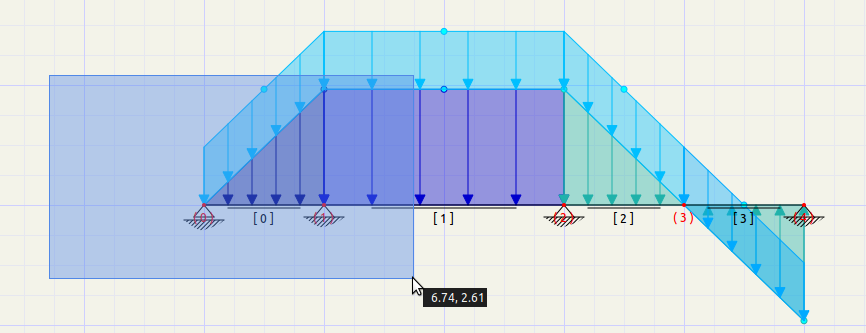
\includegraphics[width=\textwidth]{./pictures/selectionrect.png}
\caption{Selecting a Rect}
\label{pic:selectionrect}
\end{center}
\end{figure}


\subsection{Autozoom and scaling}
\begin{minipage}[h]{7cm}
\begin{figure}[H]
\begin{center}
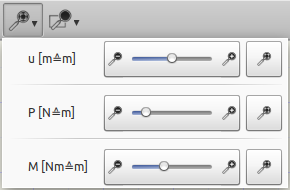
\includegraphics[scale=0.6]{./pictures/scaletoolbar.png}
\caption{Scaling menu}
\label{pic:scaletoolbar}
\end{center}
\end{figure}
\end{minipage}
\begin{minipage}[h]{\textwidth-7cm}
A short click on this button activates the auto zoom. The GraphicViews are adjusted so that the current structure fits well into them.\\
Keep the mouse button pressed to get access to the menu shown in figure~\ref{pic:scaletoolbar}. You see a slider for the scaling of the deformation, a slider for forces and a slider for moments. The slider can be used to adjust the scaling of these in the GraphicsViews. The magnifying glasses left and right from the slider can be pressed to adjust the scaling too. The buttons on the right side of the menu active the autozoom for the corresponding physical values. You can also adjust zoom with the mouse wheel and the mouse wheel in combination with some modifiers. See section~\ref{sec:graphical} and section~\ref{ssec:miscsettings} for more information about the zooming with the mousewheel.
\end{minipage}

\subsection{Calculate}

\subsection{Snap}

\subsection{Windows}

\section{GraphicView}
\label{sec:graphical}

\section{Sidebar}
\label{sec:sidebar}

\subsection{Tree Representation}
\label{ssec:tree}

\subsection{Library Widget}
\label{ssec:library}

\subsection{Prining Widget}
\label{ssec:printingwidget}

\subsection{Console}
\label{ssec:console}


\section{Start Tab}
\label{sec:starttab}

This page is the first you see when you start \Colin. Also, this page pops up when you press the "+" in the tabbar(section~\ref{sec:tabbar}), the entry in the menu (\textit{file} $\rightarrow$ \textit{new tab}) or the corresponding shortcut (Ctrl+T). 
\begin{figure}[H]
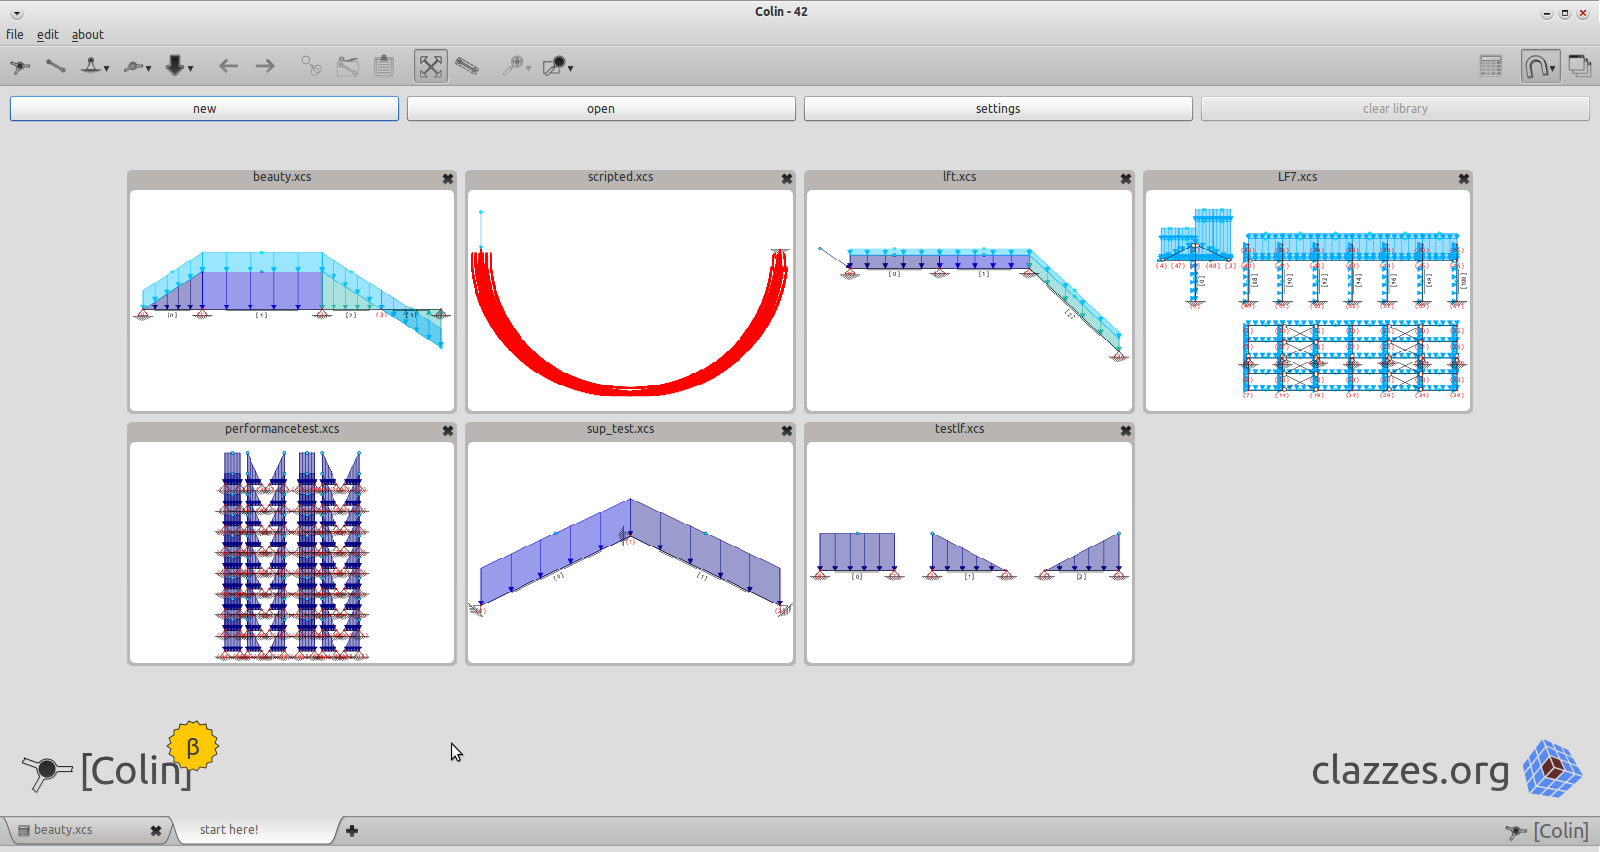
\includegraphics[width=\textwidth]{./pictures/startpage.png}
\caption{startpage}
\label{pic:startpage}
\end{figure}
Here you find the last opened files as previews. Click on the previews to open the corresponding files or to change to the corresponding tab when the file is already open. Click on the cross (top, right) to remove this preview from the startpage. You can also create new files (Button \textit{new}), open files (Button \textit{open}) access the settings (Button \textit{settings}) and clear the library when no file is open (Button \textit{clear library}).

\section{Settings}
\label{sec:settings}
Here you find all the settings. You can reach this page from the startpage, the menu (\textit{edit} $\rightarrow$ \textit{settings}) or the corresponding shortcut (Ctrl+Space). This page is divided in three pages:
\begin{itemize}
	\item color settings
	\item shortcut settings
	\item miscellaneous settings
\end{itemize}\\
You can access the pages using the buttons on top of this page. Restore the settings which \Colin has at the beginning by pressing the Button \textit{restore settings}. 

\subsection{Color Settings}
Here you can change the colors used to draw the Structure in the GraphicView. Click on a Button on the left side and change the color in the dialog besides them.
\begin{figure}[H]
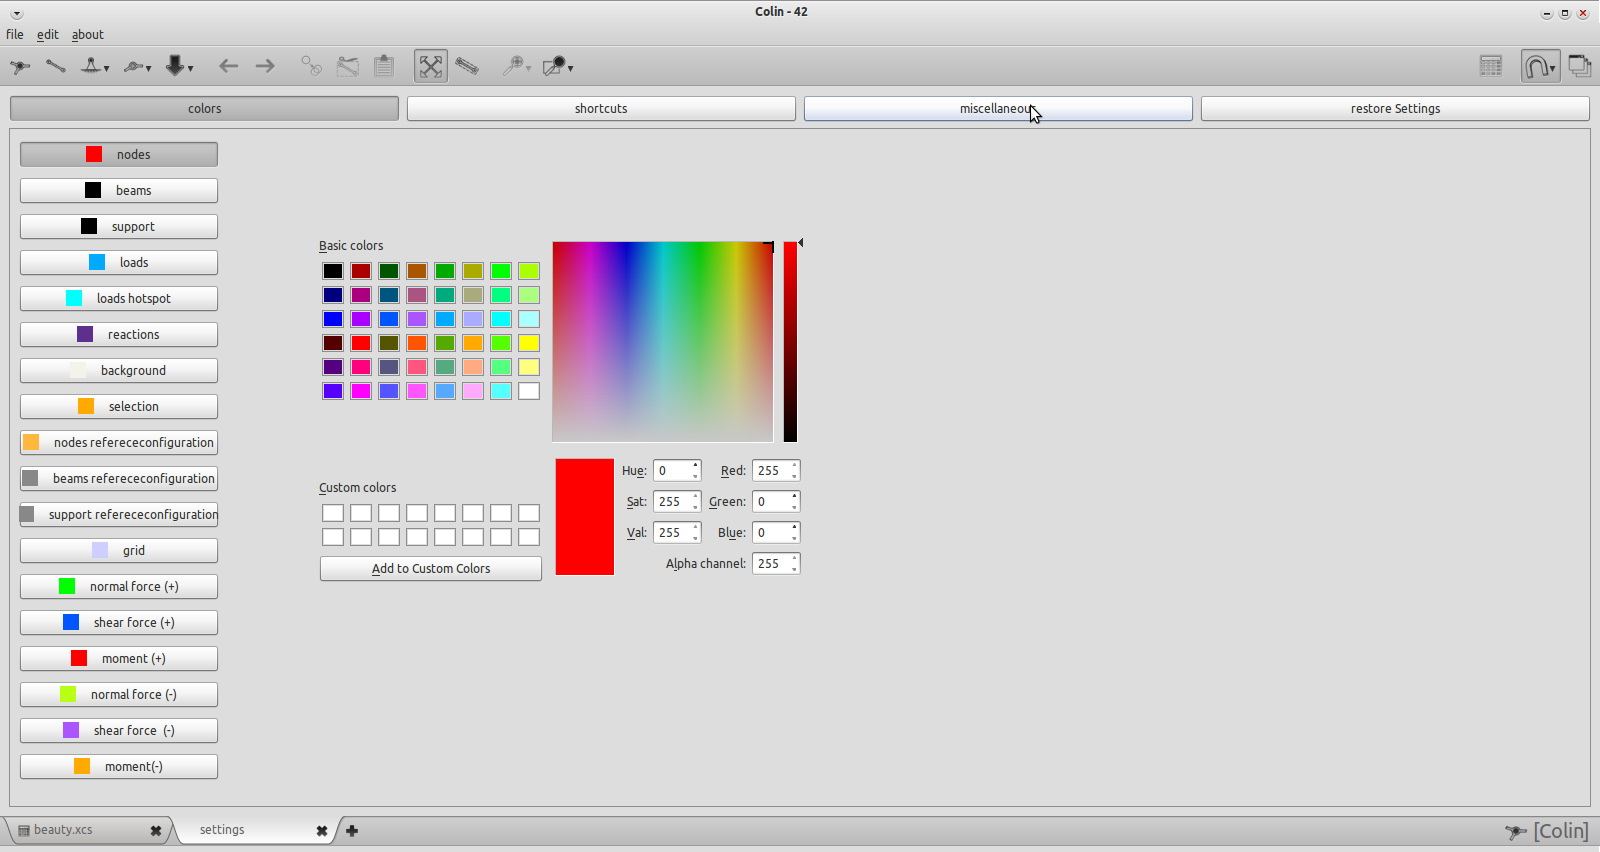
\includegraphics[width=\textwidth]{./pictures/settings_colors.png}
\caption{color settings}
\label{pic:colorsettings}
\end{figure}


\subsection{ShortCut Settings}
Here you can change the shortcuts of all actions. Click the Button \textit{change} to edit a shortcut. A line with an editable text should appear as in figure~\ref{pic:editshortcut}.\\
You can now enter the new shortcut. Use "+" to combine more keys. Use \texttt{Ctrl} for Control key, \texttt{Shift} for Shift key, \texttt{Alt} for Alt key, \texttt{Tab} for Tab key, \texttt{Space} for the Spacebar. Press \textit{Enter} to finish the editing.\\
You can restore the previous shortcut with the Button \textit{restore} besides the action.

\begin{figure}[H]
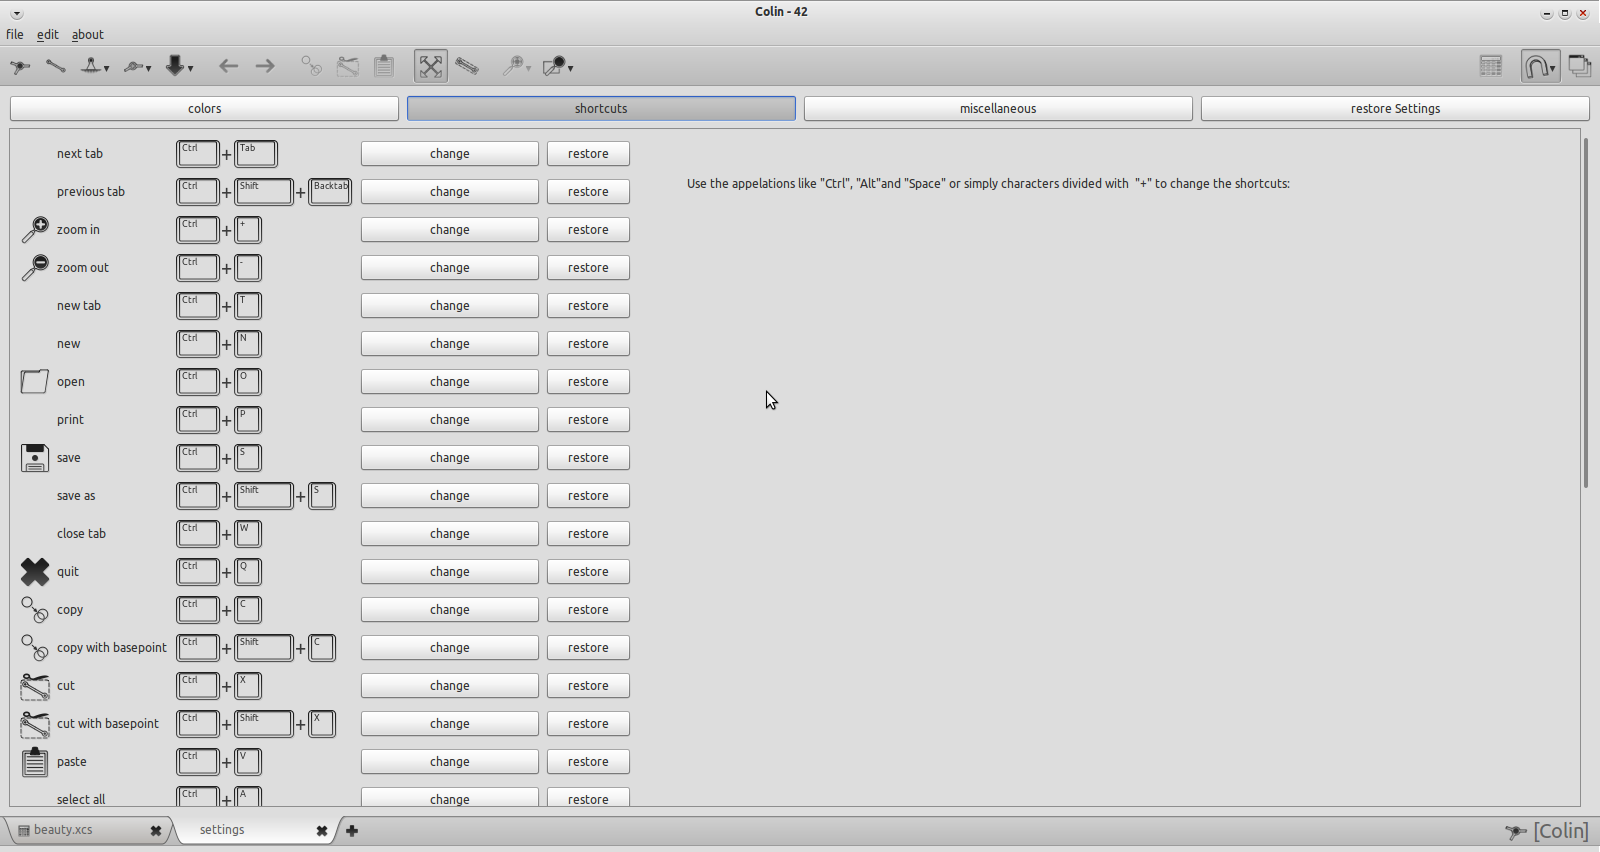
\includegraphics[width=\textwidth]{./pictures/settings_shortcuts.png}
\caption{shortcut settings}
\label{pic:shortcutsettings}
\end{figure}

\begin{figure}[H]
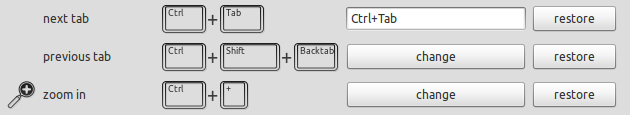
\includegraphics[width=\textwidth]{./pictures/editshortcut.png}
\caption{edit shortcut}
\label{pic:editshortcut}
\end{figure}

\subsection{Miscellaneous Settings}
\label{ssec:miscsettings}
Here you gain access to other settings:
\begin{itemize}
	\item language: set the language. Chose guess to use the same language as your operation system.
	\item mouse wheel: set modifiers for the mouse wheel which are used to scale forces, deformations and moments in the GraphicView.
	\item units: set the units which appear in the GUI and the precision of numeric values which appear in the GUI.
	\item drawing: some basic drawing settings as antialising, scaling and the appeareance of tooltips.
\end{itemize}
\begin{figure}[H]
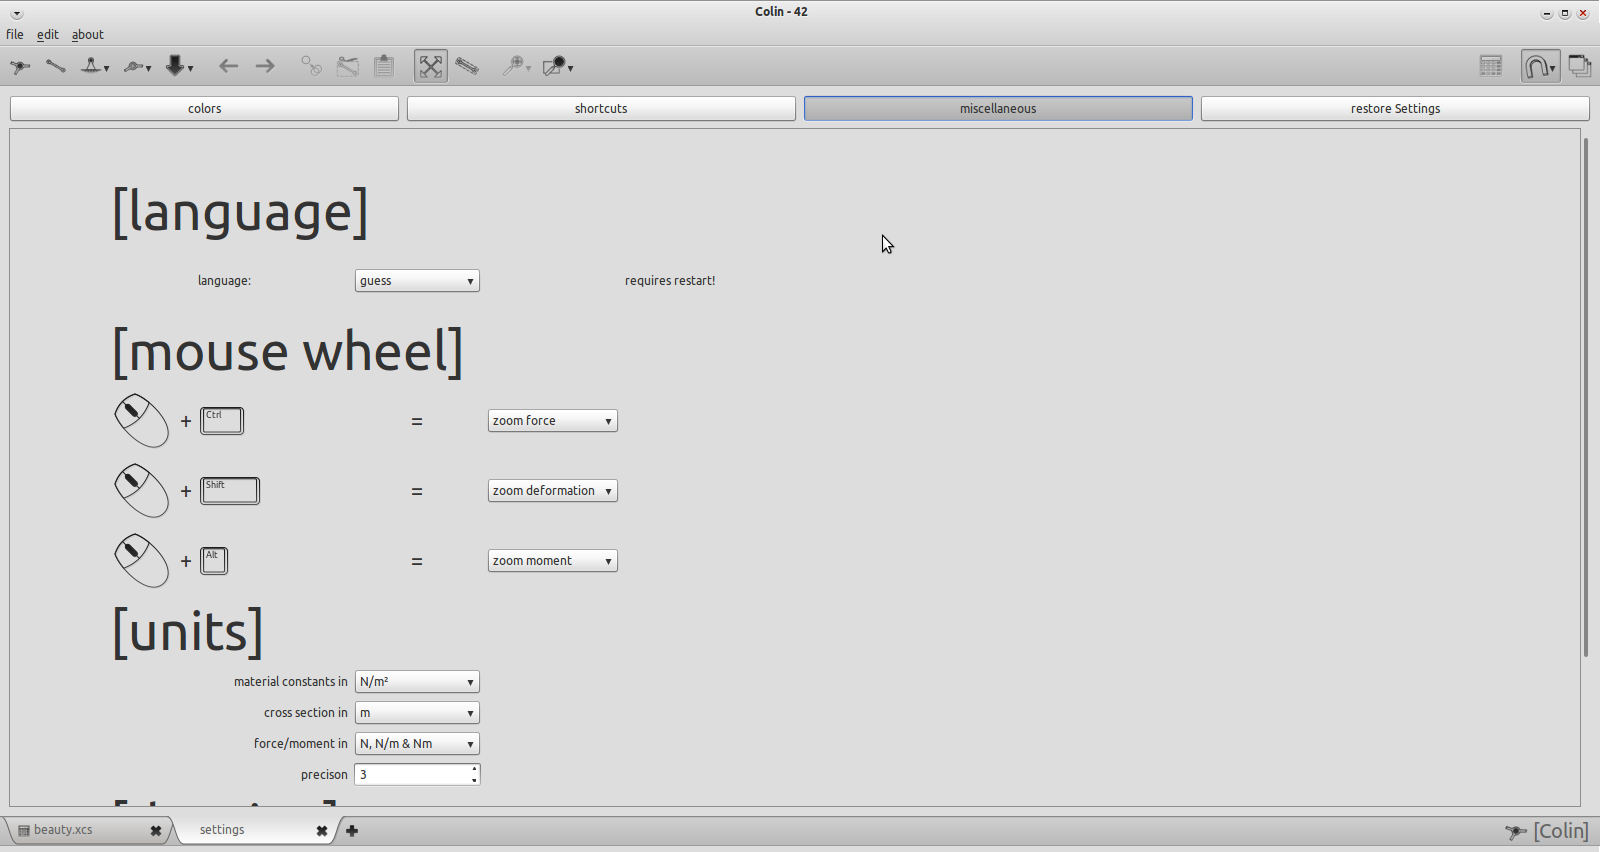
\includegraphics[width=\textwidth]{./pictures/settings_misc.png}
\caption{miscellaneous settings}
\label{pic:miscsettings}
\end{figure}

\chapter{Create and Manipulate!}
\label{cha:create}

\chapter{Script Engine}
\label{cha:scripting}

\chapter{Colin Data Format}
\label{cha:data}

\chapter{Calculation}
\label{cha:calculation}

\chapter{Compiling}
\label{cha:compile}

\chapter{Valgrind hints}
\label{cha:valgrind}
Valgrind is memory check tool and threading check tool for Unix. It detects memory leaks, uninitialized memory, corrupt reads and writes on memory, running conditions, dead locks etc.\footnote{\url{http://valgrind.org/}}\\
You should find a valgrind package in your distributors repository. On a Debian based Linux you can install it by typing the following in a terminal:

\begin{lstlisting}[frame=single, breaklines=true, basicstyle=\small]
sudo apt-get install valgrind
\end{lstlisting}

You than can run valgrind as follows:
\begin{lstlisting}[frame=single, breaklines=true, basicstyle=\small]
valgrind --leak-check=full ./Colin -graphicssystem raster
\end{lstlisting}

To remove warnings detected in libraries such as Qt, add suppression files to the valgrind parameters. The valgrind folder in the SVN repository contains a bash script to download the supression file for the gnome environment. Run the following in the valgrind folder to get it:
\begin{lstlisting}[frame=single, breaklines=true, basicstyle=\small]
./get_supp.sh
\end{lstlisting}

Run valgrind afterwards as follows in the Debug folder:
\begin{lstlisting}[frame=single, breaklines=true, basicstyle=\small]
valgrind --leak-check=full --suppressions=../valgrind/libh3dtoolkit.supp ./Colin -graphicssystem raster
\end{lstlisting}

You can add warnings to the supression file if you are sure they do not affect the right execution application.



\chapter{Get Involved}
\label{cha:involved}

\Colin is a hobby for us. We work on this project in our free time. And we need help, there is a lot of work waiting ;). If you want to improve \Colin you are grateful welcome. We will try our best to help you start! Just contact us via mail\footnote{\href{mailto:matthias.rauter@iteg.at}{matthias.rauter@iteg.at}}, twitter\footnote{\url{twitter.com/mattis_colin}} or wiki\footnote{\url{confluence.clazzes.org/}}.\\
Please note that the license you chose must be compatible with the GNU General Public License.


\section{Feedback}
Let us know what you think of \Colin, what you are waiting for, what you would change! Found a bug?
Then you are welcome to use your bugtraker at clazzes.org\footnote{\url{https://jira.clazzes.org/}} or contact us!

\section{Documentation}
This documentation sucks? Yeah, i know... :(\\
However, you can also find this document in the doc folder in our SVN repistory! Feel free to improve it!

\section{Translate}
Currently there are translations for German and Italian available. The native language of \Colin is English.
\Colin uses the Qt Framework to translate menus, tooltips, etc. You can find translation files in the source repository in the SVN repository. You can open and edit them using Qt Linguist\footnote{should be available in the software center on Linux and here for Windows and Mac OS X:\url{http://qt-apps.org/content/show.php/Qt+Linguist+Download?content=89360}}.

\section{Artwork}
You can draw icons, backgrounds or splashscreens? We are searching a guy/girl like you! Contact us!

\section{Code}
As mentioned before, the code is availibe in our SVN\footnote{again the url: \url{http://svn.clazzes.org/svn/colin/}}. You should contact us to get write access to the repository. Of course you can also send us patches via mail, bugtracker or wiki!

\chapter{Changelog}

\paragraph{Version 0.2.0-0}
\begin{compactitem}
\item added Basic Load Sets
\item added Combined Load Sets
\item elements can now be created in the treeview
\item fixed some problems with the tooltips
\item using native selection rectangles
\item added a dialog for printing of the protocol
\item renewed the sidebar
\item added javscript engine
\item added a console
\end{compactitem}
\texttt{Matthias Rauter <matthias.rauter@student.uibk.ac.at>  Mon, 28 Nov 2011 11:01:00 +0100}
\paragraph{Version 0.1.10-0}
\begin{compactitem}
\item cosmetical fixes for windows 7
\item fixed a bug in the calculation of double loads
\end{compactitem}
\texttt{Matthias Rauter <matthias.rauter@student.uibk.ac.at>  Son, 6 Nov 2011 19:55:00 +0100}
\paragraph{Version 0.1.9-0}
\begin{compactitem}
\item edit material dialog now uses the right prefix
\item changed compiler infracstructure for windows
\item some fixes on the multibutton
\item using exception in calculation
\item fixed some valgrind warnings 
\item fixed memory leaks
\end{compactitem}
\texttt{Matthias Rauter <matthias.rauter@student.uibk.ac.at>  Sat, 15 Okt 2011 10:54:00 +0100}
\paragraph{Version 0.1.8-2}
\begin{compactitem}
\item fixed the application icon in the system menu, try nr. 2
\end{compactitem}
\texttt{Matthias Rauter <matthias.rauter@student.uibk.ac.at>  Fre, 08 Apr 2011 23:32:00 +0100}
\paragraph{Version 0.1.8-1}
\begin{compactitem}
\item fixed the application icon in the system menu
\end{compactitem}
\texttt{Matthias Rauter <matthias.rauter@student.uibk.ac.at>  Fre, 08 Apr 2011 09:13:00 +0100}
\paragraph{Version 0.1.8-0}
\begin{compactitem}
\item added symbols in the pdf document
\item fixed a recursive paintevent
\item the snap (and tooltips) work now correct while drawing loads
\item the file tab now shows the right name
\item fixed a problem with the escape-key
\end{compactitem}
\texttt{Matthias Rauter <matthias.rauter@student.uibk.ac.at>  Mon, 04 Apr 2011 18:20:00 +0100}
\paragraph{Version 0.1.7-0}
\begin{compactitem}
\item all anticlockwise angles are now positiv
\item added [N/rad] for rotation springs. implemented in tree, menu, printer and resultwidget.
\item the right click menu for loads now shows the correct units
\item detailwidget now shows the angle of supports in grad instead of rad
\end{compactitem}
\texttt{Matthias Rauter <matthias.rauter@student.uibk.ac.at>  Sat, 26 Mar 2011 01:40:00 +0100}
\paragraph{Version 0.1.6-0}
\begin{compactitem}
\item Fixed a bug with nodal forces on beams (Colin addes some hinges while drawing). Should work now...
\item Added the possibility to add hinges to beams, not only to the beamends
\end{compactitem}
\texttt{Matthias Rauter <matthias.rauter@student.uibk.ac.at>  Thu, 17 Mar 2011 22:02:00 +0100}
\paragraph{Version 0.1.5-0}
\begin{compactitem}
\item Reaction forces of springs are now correct
\item the right click menu for beams now shows the correct unit for spring constants
\item the actions for copy, cut and delete in the right click menu for temperatures should work now
\end{compactitem}
\texttt{Matthias Rauter <matthias.rauter@student.uibk.ac.at>  Thu, 17 Mar 2011 11:22:00 +0100}
\paragraph{Version 0.1.4-0}
\begin{compactitem}
\item Fixed a bug with nodal forces on rotated nodes
\end{compactitem}
\texttt{Matthias Rauter <matthias.rauter@student.uibk.ac.at>  Tue, 15 Mar 2011 11:25:00 +0100}
\paragraph{Version 0.1.3-0}
\begin{compactitem}
\item Some bug fixes
\end{compactitem}
\texttt{Matthias Rauter <matthias.rauter@student.uibk.ac.at>  Sun, 13 Mar 2011 16:22:00 +0100}
\paragraph{Version 0.1.2-1}
\begin{compactitem}
\item Correcting the mail-address
\end{compactitem}
\texttt{Matthias Rauter <matthias.rauter@student.uibk.ac.at>  Sat, 12 Mar 2011 16:27:00 +0100}
\paragraph{Version 0.1.2-0}
\begin{compactitem}
\item Some Windows Fixes
\end{compactitem}
\texttt{Matthias Rauter <matthias.rauter@uibk.ac.at>  Tue, 08 Mar 2011 19:38:00 +0100}
\paragraph{Version 0.1.1-0}
\begin{compactitem}
\item Adding menu entry, translations
\end{compactitem}
\texttt{Matthias Rauter <matthias.rauter@uibk.ac.at>  Tue, 08 Mar 2011 15:03:00 +0100}
\paragraph{Version 0.1.0-0}
\begin{compactitem}
\item First debianization of Colin
\end{compactitem}
\texttt{Matthias Rauter <matthias.rauter@uibk.ac.at>  Tue, 08 Mar 2011 10:07:00 +0100}



%\clearpage
%\pagenumbering{roman}
%\setcounter{page}{9}
%\bibliography{./bibtex/mbac}



\end{document}

